\documentclass{article}
\usepackage{tikz}
\usetikzlibrary{automata,positioning}

\begin{document}

\begin{figure}[ht]
    \centering
    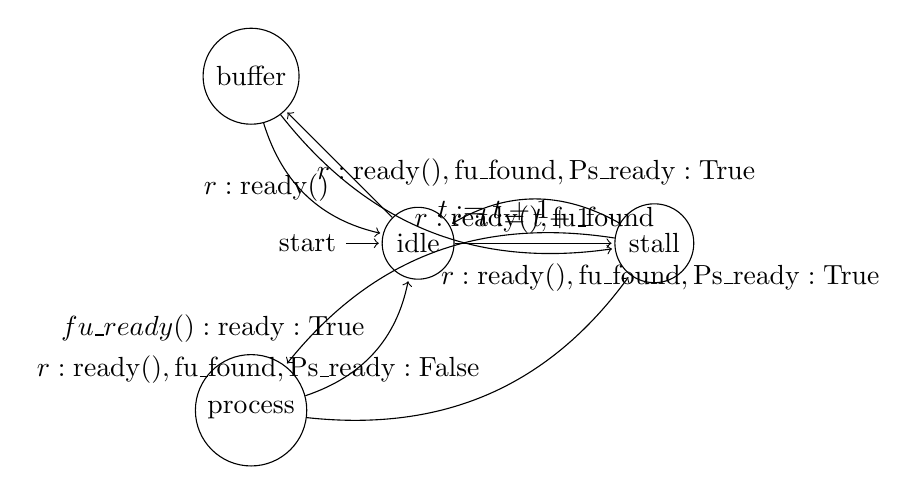
\begin{tikzpicture}[shorten >=1pt,node distance=3cm,on grid,auto]
        \node[state,initial] (q_0) {idle};
        \node[state] (q_1) [above left =of q_0] {buffer};
        \node[state] (q_2) [below left =of q_0] {process};
        \node[state] (q_3) [right =of q_0] {stall};

        \path[->]
            (q_0) edge node {$r:\mathrm{ready}()$} (q_1)
                  edge node {$r:\mathrm{ready}(),\mathrm{fu\_found}$} (q_3)
            (q_1) edge[bend right] node {$r:\mathrm{ready}(),\mathrm{fu\_found},\mathrm{Ps\_ready}:\mathrm{True}$} (q_0)
                  edge[bend right] node {$t:=t+1$} (q_3)
            (q_2) edge[bend right] node {$fu\_ready():\\\mathrm{ready}:\mathrm{True}$} (q_0)
            (q_2) edge[bend right] node {$r:\mathrm{ready}(),\mathrm{fu\_found},\mathrm{Ps\_ready}:\mathrm{False}$} (q_3)
            (q_3) edge[bend right] node {$t:=t+1$} (q_0)
            (q_3) edge[bend right] node {$r:\mathrm{ready}(),\mathrm{fu\_found},\mathrm{Ps\_ready}:\mathrm{True}$} (q_2);
    \end{tikzpicture}
    \caption{State diagram of the ACADL ExecuteStage class. The $fu$ represents any of the contained FunctionalUnits, and $ps$ represents any of the connected PipelineStages.}
\end{figure}

\end{document}